\documentclass{beamer}
 
\usepackage[utf8]{inputenc}
\usepackage{graphicx}
 
%Information to be included in the title page:
\title{Hacking on SPARC}
\author{Mohammad Yazdani}
\institute{CS 850}
\date{2018}
 
\begin{document}
 
\frame{\titlepage}
 
\begin{frame}
\frametitle{Where to begin?}
The process of booloading a toy kernel on SPARC is partly easy, partly interesting and mostly challenging.
\begin{itemize}
    \item OpenFirmware: Boot sequence is determined by a 512 byte table in the start of memory space.
    \item A position-independent binary has to be loaded into memory.
    \item In the binary, the loader starts with the text section
    \item Our boot.S determines the position of a string we want to print, and the printing function.
    \item Sets string pointer and length as 1st and second arguments and then calls the function.
\end{itemize}
\end{frame}

\begin{frame}
    \frametitle{Now: ld}
    Then we need to tell ld to:
    \begin{itemize}
        \item Kickout the headers
        \item Add a.out signature
        \item Size of our text section (comes after header)
    \end{itemize}
\end{frame}

\begin{frame}
    \frametitle{After many hours}
    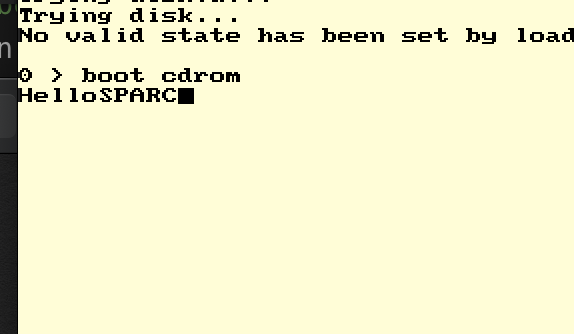
\includegraphics{sshot.png}
\end{frame}

\begin{frame}
    \frametitle{What I learned and what was interesting:}
    \begin{itemize}
        \item Compilers matter: I faced a lot of problems being able to get the right assembler and the right compiler. In the process of figuring out the bootloader I started to get more and more interested in diving deeper on compilers as an integral part of systems dev.
        \item Compared to what I read on boot loaders for other architectures, the SPARC boot loader is rather more straight forward. The basic process is figuring out your entry point, pointing to something you want to do, return from it and loop.
    \end{itemize}
\end{frame}

\end{document}